%============================================================================%
%
%	DOCUMENT DEFINITION
%
%============================================================================%

%we use article class because we want to fully customize the page and don't use a cv template
\documentclass[10pt,a4paper]{article}

%----------------------------------------------------------------------------------------
%	ENCODING
%----------------------------------------------------------------------------------------

% we use utf8 since we want to build from any machine
\usepackage[utf8]{inputenc}

%----------------------------------------------------------------------------------------
%	LOGIC
%----------------------------------------------------------------------------------------

% provides \isempty test
\usepackage{xifthen}

%----------------------------------------------------------------------------------------
%	FONT BASICS
%----------------------------------------------------------------------------------------
\usepackage[default]{raleway}

% set font default
\renewcommand*\familydefault{\sfdefault}
\usepackage[T1]{fontenc}

% more font size definitions
\usepackage{moresize}

% ragged right that still hyphenates, used in the narrow left column
\usepackage{ragged2e}

%----------------------------------------------------------------------------------------
%	PAGE LAYOUT  DEFINITIONS
%----------------------------------------------------------------------------------------

% page outer frames (debug-only)
% \usepackage{showframe}

% we use paracol to display breakable two columns
\usepackage{paracol}

% define page styles using geometry
\usepackage[a4paper]{geometry}

% remove all possible margins
\geometry{top=1cm, bottom=1cm, left=1cm, right=1cm}

\pagestyle{empty}

% indentation is zero
\setlength{\parindent}{0mm}

%----------------------------------------------------------------------------------------
%	TABLE / ARRAY DEFINITIONS
%----------------------------------------------------------------------------------------

% extended aligning of tabular cells
\usepackage{array}

% tighter lists so a single bullet does not insert a float-sized gap
\usepackage{enumitem}

%----------------------------------------------------------------------------------------
%	GRAPHICS DEFINITIONS
%----------------------------------------------------------------------------------------

%for header image and technology icons
\usepackage{graphicx}

%----------------------------------------------------------------------------------------
%	Color DEFINITIONS
%----------------------------------------------------------------------------------------
\usepackage{color}

% primary color
\definecolor{maincol}{RGB}{ 225, 0, 0 }

% accent color, secondary
% \definecolor{accentcol}{RGB}{ 250, 150, 10 }

% dark color
\definecolor{darkcol}{RGB}{ 70, 70, 70 }

% light color
\definecolor{lightcol}{RGB}{245,245,245}


% Package for links, must be the last package used
\usepackage[hidelinks]{hyperref}
\hypersetup{%
  pdftitle={Clayton Asada Resume},%
  pdfauthor={Clayton Asada},%
  pdfsubject={Senior Software Engineer},%
  pdfkeywords={Clayton Asada, software engineer, Java, AWS, Kubernetes}%
}

% returns minipage width minus two times \fboxsep
% to keep padding included in width calculations
% can also be used for other boxes / environments
\newcommand{\mpwidth}{\linewidth-\fboxsep-\fboxsep}


%============================================================================%
%
%	CV COMMANDS
%
%============================================================================%

%----------------------------------------------------------------------------------------
%	 CV LIST
%----------------------------------------------------------------------------------------

% one bullet per job; keep the article indent, drop the default list gap
\newcommand{\cvlist}[1]{%
	\begin{itemize}[topsep=3pt,partopsep=0pt,parsep=0pt,itemsep=2pt,leftmargin=2.5em]%
		#1%
	\end{itemize}%
}

%----------------------------------------------------------------------------------------
%	 CV TEXT
%----------------------------------------------------------------------------------------

% full-width text. the inner parbox keeps \\ inside headings from ending the row.
\newcommand{\cvtext}[1]{%
	\begin{tabular}{@{}p{\linewidth}@{}}%
		\parbox{\linewidth}{#1}%
	\end{tabular}%
}

%----------------------------------------------------------------------------------------
%	CV RIGHT SECTION
%----------------------------------------------------------------------------------------

% Renders a CV section headline with a short underline in the main color.
% param 1: section title
\newcommand{\cvsection}[1]{%
	\vspace{10pt}%
	\cvtext{%
		\textbf{\LARGE{\textcolor{darkcol}{\uppercase{#1}}}}\\[-6pt]%
		\textcolor{maincol}{\rule{0.1\textwidth}{2pt}}\\%
	}%
	\vspace{0pt}%
}

%----------------------------------------------------------------------------------------
%	CV LEFT SECTION
%----------------------------------------------------------------------------------------

% Renders a sidebar section headline. same underline length as the right column.
% param 1: section title
\newcommand{\cvleftsection}[1]{%
	\vspace{9pt}%
	\cvtext{%
		\textbf{\large{\textcolor{darkcol}{\uppercase{#1}}}}\\[-6pt]%
		\textcolor{maincol}{\rule{0.1\textwidth}{2pt}}\\%
	}%
	\vspace{-3pt}%
}

%----------------------------------------------------------------------------------------
%	META SKILL
%----------------------------------------------------------------------------------------

% name on the left, years flush right. ragged so narrow labels wrap on spaces.
% param 1: name of the skill / tech / etc.
% param 2: level (for example in years)
\newcommand{\cvother}[2]{%
	\begin{tabular*}{\linewidth}{@{}>{\raggedright\arraybackslash}p{0.68\linewidth}@{\extracolsep{\fill}}r@{}}%
		\textcolor{black}{\textbf{#1}} & \textcolor{maincol}{#2}%
	\end{tabular*}%
}

%----------------------------------------------------------------------------------------
%	 CV EVENT
%----------------------------------------------------------------------------------------

% the whole entry is one parbox so a page break cannot separate the title from its bullets.
% param 1: time-frame i.e. Sep 14 - Jan 15 etc.
% param 2: event name (job position etc.)
% param 3: Customer, Employer, Industry
% param 4: Short description (optional)
% param 5: work done (optional)
% param 6: technologies include (optional)
% param 7: achievements (optional)
\newcommand{\cvevent}[7]{%
	\parbox{\linewidth}{%
		\begin{tabular*}{\linewidth}{@{}p{0.62\linewidth}@{\extracolsep{\fill}}r@{}}%
			\textcolor{black}{\textbf{#2}} & \colorbox{maincol}{\makebox[0.35\mpwidth]{\textcolor{white}{#1}}} \\%
			\textcolor{maincol}{\textbf{#3}} & \\%
		\end{tabular*}\\[5pt]%
		\ifthenelse{\isempty{#4}}{}{%
			\cvtext{#4}\\%
		}%
		\ifthenelse{\isempty{#5}}{}{%
			#5%
		}%
		\ifthenelse{\isempty{#6}}{}{%
			\vspace{4pt}%
			\textbf{Technology Stack:}\par
			\vspace{2pt}%
			#6\par
		}%
		\ifthenelse{\isempty{#7}}{}{%
			\vspace{3pt}%
			\textbf{Achievements:}\par
			#7%
		}%
	}%
	\vspace{15pt}%
}

%----------------------------------------------------------------------------------------
%	 CV MINI EVENT
%----------------------------------------------------------------------------------------

% title, date, and organization only.
% param 1: time-frame
% param 2: event name
% param 3: customer, employer, etc.
\newcommand{\cvminievent}[3]{%
	\parbox{\linewidth}{%
		\begin{tabular*}{\linewidth}{@{}p{0.55\linewidth}@{\extracolsep{\fill}}r@{}}%
			\textcolor{black}{\textbf{#2}} & \colorbox{maincol}{\makebox[0.4\mpwidth]{\textcolor{white}{#1}}} \\%
			\textcolor{maincol}{\textbf{#3}} & \\%
		\end{tabular*}%
	}%
}

%----------------------------------------------------------------------------------------
%	 CV META EVENT
%----------------------------------------------------------------------------------------

% Renders a CV event on the sidebar.
% param 1: title
% param 2: subtitle (optional)
% param 3: customer, employer, etc. (optional)
% param 4: info text (optional). set ragged because the column is narrow.
\newcommand{\cvmetaevent}[4]{%
	\vspace{-7pt}%
	\textcolor{maincol}{\cvtext{\textbf{\begin{flushleft}#1\end{flushleft}}}}\\[-5pt]%
	\ifthenelse{\isempty{#2}}{}{%
		\textcolor{darkcol}{\cvtext{\textbf{#2}}}\par
	}%
	\ifthenelse{\isempty{#3}}{}{%
		\cvtext{\textcolor{darkcol}{#3}}\\%
	}%
	\cvtext{\RaggedRight #4}\\[-25pt]%
	\vspace{27pt}%
}

%---------------------------------------------------------------------------------------
%	QR CODE
%----------------------------------------------------------------------------------------

% centered LinkedIn QR. param 1: fraction of the column width, from 0 to 1
\newcommand{\cvqrcode}[1]{%
	\begin{center}%
		\href{https://www.linkedin.com/in/clayton-asada-46986ab1/}{%
			
\includegraphics[width=#1\linewidth]{images/linkedinQR.png}%
		}%
	\end{center}%
}

% one technology mark plus its label, at the icon's real aspect ratio
\newcommand{\cvicon}[2]{%
	\includegraphics[height=.5cm,keepaspectratio]{#1}\,#2%
}

% five icon labels spread across the column
\newcommand{\cvicons}[5]{%
	\begin{tabular*}{\linewidth}{@{}l@{\extracolsep{\fill}}llll@{}}%
		#1 & #2 & #3 & #4 & #5%
	\end{tabular*}%
}


%============================================================================%
%
%	DOCUMENT CONTENT
%
%============================================================================%
\begin{document}
\columnratio{0.29}
\setlength{\columnsep}{2.2em}
\setlength{\columnseprule}{4pt}
\colseprulecolor{lightcol}
\begin{paracol}{2}
\begin{leftcolumn}
%---------------------------------------------------------------------------------------
%	META IMAGE
%----------------------------------------------------------------------------------------
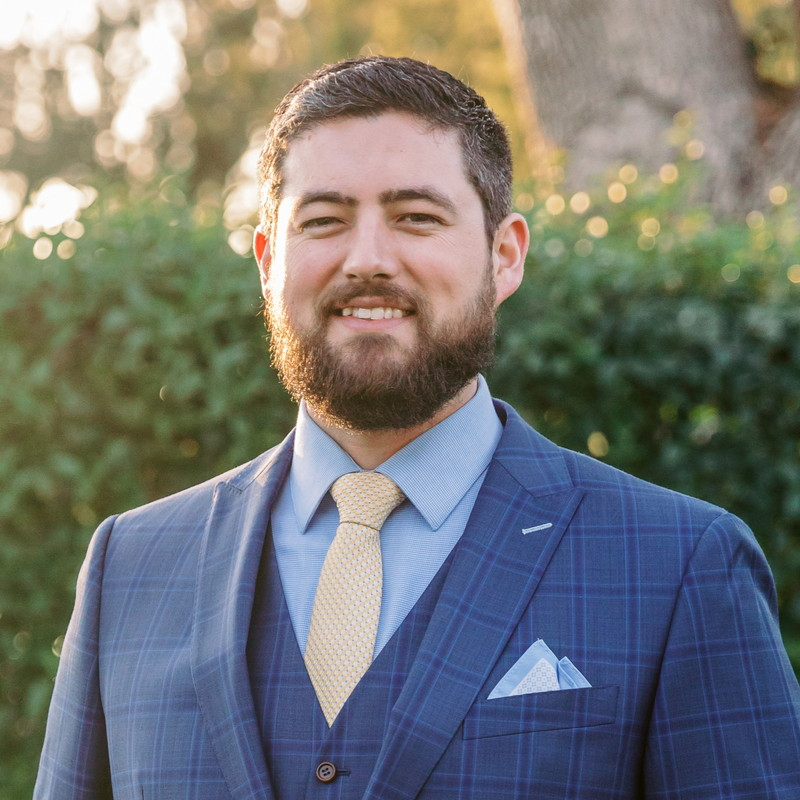
\includegraphics[width=\linewidth]{images/headshot-print.jpg}

%---------------------------------------------------------------------------------------
%	META SKILLS
%----------------------------------------------------------------------------------------
\cvleftsection{Languages} \\
\cvother{Java 13+}{5 yrs}
\cvother{SQL}{5 yrs}
\cvother{JavaScript}{9 mo}
\cvother{Python}{1+ yrs}

\cvleftsection{TECHNOLOGIES} \\
\cvother{Amazon Web Services (AWS)}{5 yrs}
\cvother{Kubernetes}{2 yrs}
\cvother{Docker/Podman}{2 yrs}

\cvleftsection{TOOLS} \\
\cvother{IntelliJ}{3 yrs}
\cvother{VS Code}{2 yrs}
\cvother{NeoVim}{3+ yrs}
\cvother{Atlassian Suite}{5 yrs}

%---------------------------------------------------------------------------------------
%	EDUCATION
%----------------------------------------------------------------------------------------
\cvleftsection{EDUCATION}

\cvmetaevent
{08/15/2022 - 05/15/2024}
{M.S. Computer Science}
{C.S.U., Long Beach \hfill \textcolor{maincol}{\textbf{GPA: 4.0}}}
{Computer Science Master’s Program with thesis on AI/ML. I graduated 2nd in my class and introduced a novel dropout technique in my thesis, ’Sector-Wise Dropout’.}

\cvmetaevent
{08/15/2015 - 05/15/2020}
{B.S. Computer Science}
{C.S.U., Long Beach}
{}

\vfill\null
\cvqrcode{0.6}
\end{leftcolumn}
\begin{rightcolumn}
%---------------------------------------------------------------------------------------
%	TITLE  HEADER
%----------------------------------------------------------------------------------------
\noindent\colorbox{darkcol}{%
\begin{minipage}[c][3.5cm][c]{\mpwidth}
	\begin{center}
		\HUGE{\textbf{\textcolor{white}{\uppercase{Clayton Asada}}}}\\[-24pt]
		\textcolor{white}{\rule{0.3\textwidth}{1.25pt}}\\[8pt]
		\large{\textcolor{white}{Plano, TX --- \href{tel:+19168016154}{(916)~801-6154} --- \href{mailto:Casada94@gmail.com}{Casada94@gmail.com}}}
	\end{center}
\end{minipage}}\\[14pt]
\vspace{-12pt}

%---------------------------------------------------------------------------------------
%	PROFILE
%----------------------------------------------------------------------------------------
\cvsection{PROFILE}

\cvtext{I'm a highly motivated, results-driven software engineer with a strong background in Java development and cloud technologies. I thrive in dynamic environments, consistently delivering innovative solutions that enhance system performance and drive business growth.}

%---------------------------------------------------------------------------------------
%	WORK EXPERIENCE
%----------------------------------------------------------------------------------------
\cvsection{WORK EXPERIENCE}

\cvevent
	{06/2024 - Present}
	{Senior Software Engineer}
	{Raytheon}
	{Modernize, enhance, and maintain mission critical applications. Incorporating new technologies and libraries to deliver new features and/or improve readability, testability, and maintainability.}
	{\cvlist{%
		\item Bringing a heavy emphasis on code quality, my contributions have led to improved maintainability and reduced technical debt across multiple applications.%
	}}
	{\cvicons
		{\cvicon{icons/icons8-spring-boot-120.png}{Spring Boot}}
		{\cvicon{icons/gradle-icon.png}{Gradle}}
		{\cvicon{icons/cucumber_120.png}{Cucumber}}
		{\cvicon{icons/icons8-kubernetes-96.png}{Kubernetes}}
		{\cvicon{icons/icons8-linux-96.png}{Linux}}%
	}
	{\cvlist{%
		\item Became the subject matter expert and single largest contributor to a multi-project cross-team Gradle 2 to Gradle 8 migration.%
	}}

\cvevent
	{07/2024 - 09/2025}
	{Software Engineer}
	{U.S. Department of Defense}
	{Fullstack development incorporating new technologies and libraries to deliver new features and/or improve readability, testability, and maintainability.}
	{}
	{\cvicons
		{\cvicon{icons/icons8-spring-boot-120.png}{Spring Boot}}
		{\cvicon{icons/icons8-react-96.png}{React}}
		{\cvicon{icons/icons8-amazon-web-services-120.png}{AWS}}
		{\cvicon{icons/icons8-mysql-logo-120.png}{MySQL}}
		{\cvicon{icons/icons8-linux-96.png}{Linux}}%
	}
	{\cvlist{%
		\item Guided by user feedback, I created a feature to help users quickly identify the topics and context of their next task, which improved their efficiency and task throughput.%
	}}

\cvevent
	{03/2021  -  07/2024}
	{Java Developer}
	{Tata Consultancy Services: Experian}
	{}
	{}
	{}
	{\cvlist{%
		\item My Hackathon idea, inspired by customer conversions, led to implementation, completed by me, which increased yearly revenue by ~\$800,000 (16\%)%
	}}

\cvminievent
	{07/2012  -  09/2015}
	{Electrical Systems Technician}
	{United States Marine Corps}

\end{rightcolumn}
\end{paracol}
\end{document}
